%(sub-systems and dependencies between them)

\begin{center}
	 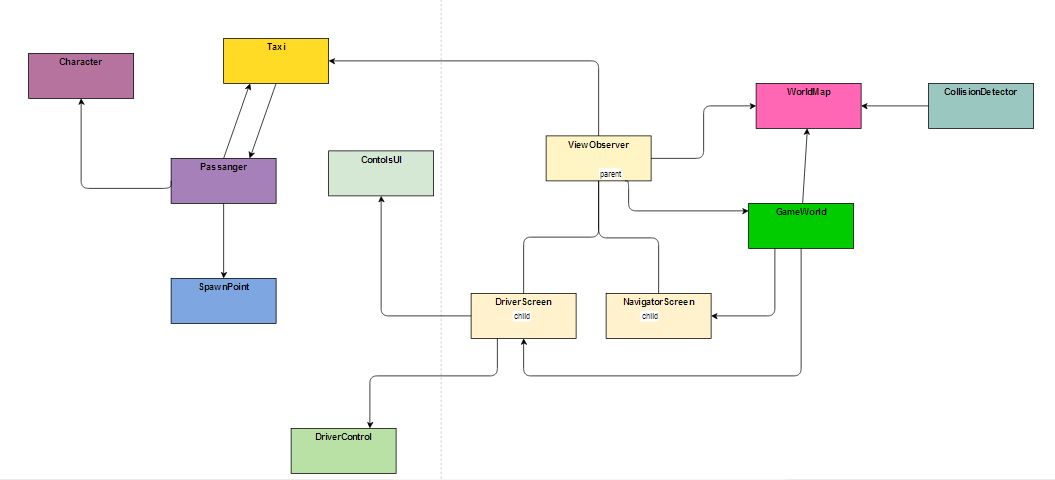
\includegraphics[width=130mm]{./images/UML2.png}

\end{center}


The architecture of the system is divided into subsystems. These subsystems are the Game Model, the Driver Interface, the Navigator Interface and the Network Interface. All subsytems will be explained in this section.

\begin{description}
	
\item[The Game Model] \hfill \\
The Game Model consists of the game world and all data related to the game. The actual game takes place in this subsystem. All other subsystems are interfaces that are used to alter the game model.

\item[The Driver Interface]  \hfill \\
This is one of the two interfaces that will be directly used by the players to interact with the Game Model. The Driver Interface enables the user to see the car and its direct surroundings. It also gives the user the means to controll the car (steering and acceleration). 

\item[The Navigator Interface]  \hfill \\
The second way for players to interact with the Game Model is the Navigator Interface. This interface gives the user an overview of the game world in the form of a map. This enables the user of this interface to (verbally) guide the user using the Driver Interface through the game world. The Navigator Interface can be used to interact with the Game Model through the activation of powerups, which will alter specific parts of the game world.

\item[The Network Interface]  \hfill \\
This interface is used to connect players with eachother. It is responsible for the connection of the two players within each team as well as the connection between all the teams. The Network Interface is also responsible for the concurrency between all Game Models.

\end{description}
